% !TEX root =  ../main.tex
\section{MaxOnlines}

\subsection{Definition}

\subsubsection{Signature} \cstr{maxOnlines(s : set<server>, n : number)}

\begin{itemize}
\item \cstr{s} : a non-empty set of servers for a meaningful constraint.
\item \cstr{n} : a positive number, inferior to the number of servers in \cstr{s}.
\end{itemize}


The \cstr{maxOnlines} ensures the number of online servers in \cstr{s} is inferior or equals to \cstr{n}.

\classification{maxOnlines}{datacenter administrator}{Resource allocation}{Resource management,Power saving,Capacity planning}

\subsubsection{Usage}

This constraint deserves the control of the datacenter hosting capacity. A datacenter may
be composed of servers that differ in their hardware capacity or performance.
It may however not be possible to keep all the servers online simultaneously. As an example,
the cooling system or the power distribution unit may restrict the number of online servers due to its delivering capacity.
Licenses restrictions, such as the per-server license model of XenServer, may also limits the number of nodes that are online
simultaneously.~\cite{xen-server}

In this setting, once the maximum number of online servers reached,  turning on one additional server
to use its specificities is only allowed if an online server can be turned off in exchange.
In this setting, a datacenter administrator may then use of \cstr{maxOnlines} constraints to control the number of online servers and automatically manage their state if needed.

\subsubsection{Example}

Figure~\ref{fig: maxOnlines} depicts a sample reconfiguration between a source and a destination configuration where only servers \cstr{N1}, \cstr{N2} and \cstr{N3} are online in the source configuration.
Each VM is associated to a gray rectangle that denotes its resource usage in terms of memory and UCPU.
In the source configuration, the server \cstr{N1} was saturated has \cstr{VM4} and \cstr{VM6} were competing for the same resources. The reconfiguration process fixed this violation but also consider the following \cstr{maxOnlines} constraints:

\begin{figure}[htb]
\centering
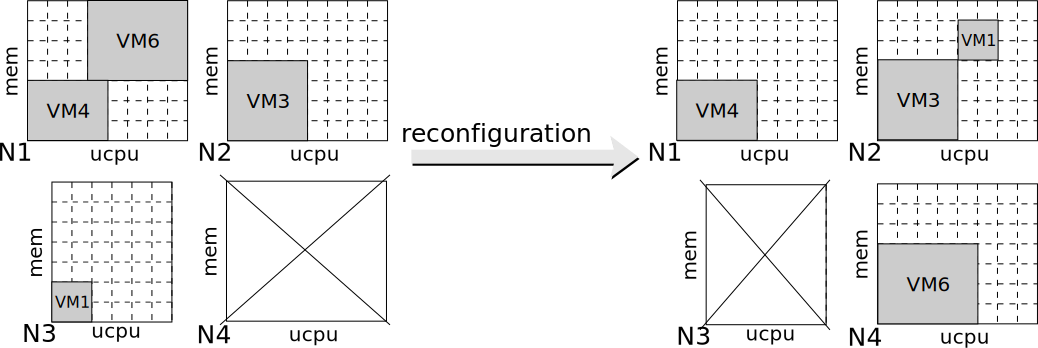
\includegraphics[width=\textwidth]{img/maxOnlines}
\caption{A reconfiguration motivated by \cstr{maxOnlines} constraints.}\label{fig: maxOnlines}
\end{figure}


\begin{itemize}

\item \cstr{maxOnlines(\{N1,N2, N3, N4\}, 3)}. This constraint was satisfied in the source configuration as three over the four
servers were in the \st{Online} state. The constraint is still satisfied in the destination configuration. \cstr{N4}�has been turned
on to host 	\cstr{VM6} but \cstr{N3} has been turned off in exchange according to the constraint specification. To be able to turned
off \cstr{N3}, \cstr{VM1} has been relocated to \cstr{N2}. Figure~\ref{fig: maxOnlines plan} depicts the associated event-based reconfiguration plan.

\begin{reconfPlan}[htb]
\centering
\begin{tabular}{ll}
\O & $\rightarrow$ relocate(VM1) \\
!relocate(VM1)\ & $\rightarrow$ halt(N3)\\
!halt(N3)\ & $\rightarrow$ boot(N4)\\
!boot(N4) & $\rightarrow$ relocate(VM6)
\end{tabular}
\caption{Event-based reconfiguration plan associated to the reconfiguration depicted in Figure~\ref{fig: maxOnlines}.}\label{fig: maxOnlines plan}
\end{reconfPlan}

\item \cstr{maxOnlines(\{N1, N3\},1)}. This constraint was not satisfied in the source configuration as the two servers were in the \st{Online}�state. The reconfiguration process fixed this violation by turning off \cstr{N3}.
\end{itemize}


\subsection{See also}

\subsubsection{Related Constraints}

\begin{itemize}
\item \cstrref{maxSpareResources}: A constraint to restrict the number of unused but available resources to a given maximum.
\end{itemize}


\printListOfInheritance{maxOnlines}
